% !TeX root = ../main.tex

\chapter{Device evaluation and dispersion analysis}% from transmission spectroscopy


In the example given in \autoref{sec:disp-comp},  a typical dispersive ring resonator has the $ D_2 $ value less than MHz, which means the frequency FSR, for example 100 GHz, is different from the next one with a MHz-level difference. It is difficult to achieve such precise measurement using traditional optical spectrum analyzer whose typical resolution is around pm, 100 MHz. The tunable laser scanning is developed to solve this problem, especially assisted by an external frequency comb \cite{Liu2016d}. 

Here, we exploit the method using laser step triggering to calibrate the real-time measured device transmission. Compared with the frequency comb or wave meter assisted spectroscopy, this method is much more convenient to deploy. By increasing the data acquisition sampling rate or altering with electric oscilloscope, the wavelength precision can be further improved.
Given the well-resonant spectrum, the dispersion information is further extracted from the transmission, in particular the resonant peaks. Such method is widely used to study the Kerr frequency comb. It is also efficient to study the frequency-entangled photon pair generation.


\section{Methods}
%\subsection{Fiber launching}

Much of related works, concerning such as photonic crystals or whispering gallery mode resonators, use prism coupling or tapered fiber coupling for coupling tunability. 
%interact the external optical filed with cavity evanescent filed though, 
In the case of integrated ring resonators, the bus wavegudies are designed in the distance of several gaps, usually varying from under-coupling to over-coupling. 
Thus, the light confined in the bus waveguide can be directly coupled inwards or outwards using appropriate optical fibers. 
In previous works \cite{Sunada2018}, both grating coupling and edge coupling were adopted. However, considering the broadband frequency conversion motivation, the edge coupling is preferred for a comparatively broader 3-dB bandwidth. 
 
Using two five-axis fiber alignment stages (Newport M-562F-XYZ \& M-562F-XYZ-LH), the device ports are aligned with two lensed fibers on both sides. The spot size of lensed fibers is 2 \um, which is not optimized to the size mentioned in \autoref{sec:chip-dicing}. 

Before any following experiments, the output port is first coupled to the infrared InGaAs camera in free space using a 20$\times$ objective lens. To align the chip input port precisely, the real-time camera images is used to adjust all the three degrees of freedom until the spot is observed explicitly on the screen. Next, by carefully rotating the palettes of polarization controller on the input side, the device coupling can be launched in either TE or TM mode. Then another lensed fiber is launched instead and aligned carefully, as the power meter reading is referred to.

In this method, the best facet-to-facet coupling efficiency is around 6 dB in the case of ligentec samples, where is optimized by mode convertors. Comparatively, a more typical facet-to-facet loss without mode convertors can be 8-9 dB.

%LS-CVD samples
It is worth mentioning that the chip arrier (SURUGA SEIKI F126) is equipped with a thermoelectric cooler (TEC), which is essential for long-time thermal stability. 
With connected to an external temperature controller, the temperature precision over device under test can be 0.1 \si{\celsius}.
To avoid moisture condensation, the TEC is set a little higher than room temperature, 30 \si{\celsius} in our case. 

%\subsection{Spectrum sweeping}

\begin{figure}
	\centering
	\includesvg[width=.9\textwidth]{trans_setup}
%	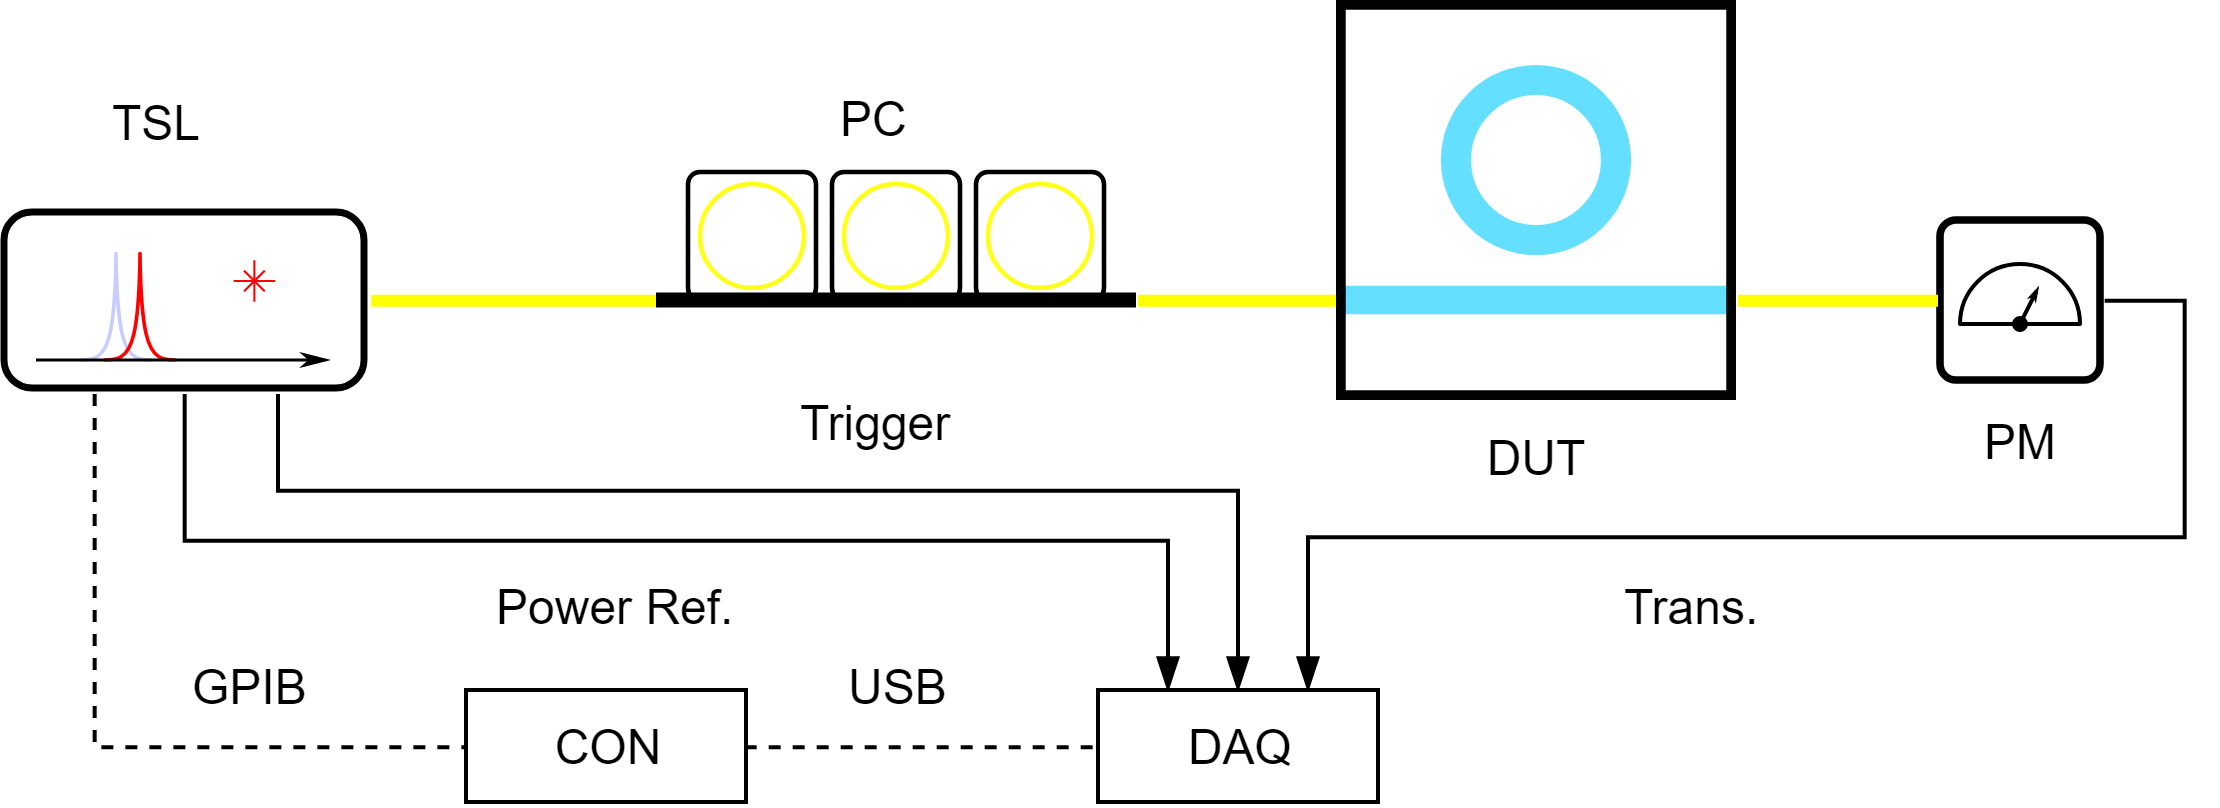
\includegraphics[width=.9\textwidth]{imgs/png/trans_setup}
	\mycaption{Setup of transmission measurement system}{TSL, tunable semiconductor laser. PC, optical fiber polarization controller. DUT, device under test. PM, power meter. DAQ, data acquisition.}
	\label{fig:transsetup}
\end{figure}

The schematic diagram of the device spectrum measurement is shown in \autoref{fig:transsetup}. 
After manual alignment, the TSL (SANTEC TSL-710) is first set to continuously sweep from 1480 nm - 1640 nm, covering the telecom S C and L bands.
The internal power reference signal and the step trigger are also generated simultaneously, which are used to calibrate the output optical power and improve wavelength scanning accuracy. The output power from device under test is measured by the power meter (Newport 2963-R). 

Compared with photon diodes, the power meter in our setup is critical to realize various range scanning.  Finally, the signals from power monitor, step trigger and device transmission are all synchronized with the data acquisition module, and then analyzed by the computer. To achieve pm-resolution spectra, transmitted power is simply divided by power reference and the step trigger are marked to interpolate wavelengths in the certain time interval.


\section{Thermal stability}

\begin{figure}
	\centering
	\includesvg[width=1\textwidth]{thermal_depen}
	%	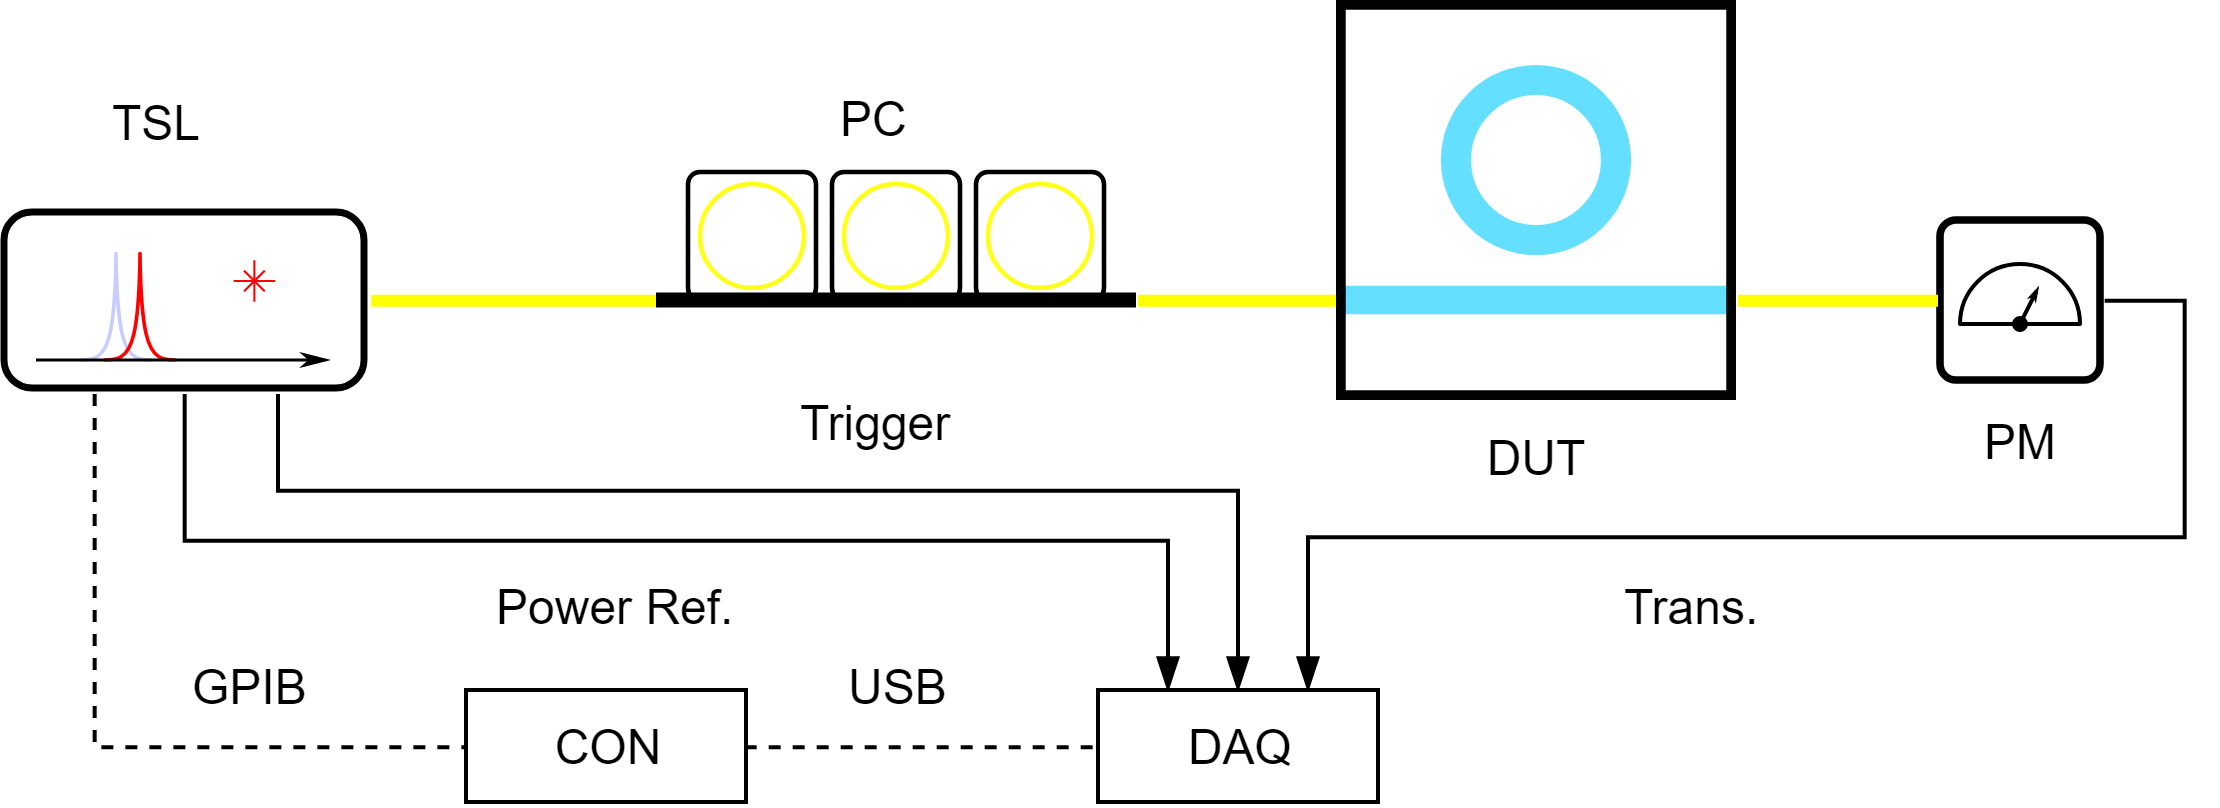
\includegraphics[width=.9\textwidth]{imgs/png/trans_setup}
	\mycaption{Thermal dependence of LP-CVD sample}{\textbf{a}. Transmission measured at three temperatures. \textbf{b}. Resonant wavelengths extracted versus temperature. The estimated thermal dependence $\dv*{\lambda}{T}$ is 23 \si{\nm/\celsius}.}
	\label{fig:thermal}
\end{figure}

Although silicon nitride is reported as high thermal conductivity material, the surrounding silicon dioxide is comparatively worse thermal conductive. Despite the room temperature fluctuation, the nonlinear phenomena usually requires high pump power intracavity, which heats the device significantly, the index change variation leads to resonance shift. Thus, the thermal sensitivity is a critical factor of nonlinear ring resonators.

For example, with the TEC set into different temperatures, the spectrum of a LP-CVD sample is then measured. Shown in \autoref{fig:thermal}a, temperature increasing leads to a obvious red-shift of the resonant peak. The wavelength range around 1630 nm is chosen for better transmission and well resonance in this device. From \autoref{fig:thermal}b, the estimated thermal dependence of resonant wavelength $\dv*{\lambda}{T}$ is 23 \si{\nm/\celsius}. In this case, if the \textit{Q}-factor of ring resonator is up to \num{10d5}, even room temperature variation can results in resonance totally mismatching at pumping wavelength.

\section{Device transmission}

Given the transmission spectra, the negative peaks are located with peak-finding algorithm, yielding not only the peak location, but also the width and prominence. These values are next used to calculate the free spectral ranges and \textit{Q}-factors. In general, due to the fabrication difference, not all the device appear resonance all around the measured band. To compensate the broken spectra, several algorithm are performed to achieve best performance of peak-finding. 

\begin{figure}
	\centering
	\includesvg[width=5in]{filt_cf}
	\mycaption{}{}
	\label{fig:spec_filt}
\end{figure}

In our technology, for the spectra with remarkable absorption illustrated in \autoref{fig:spec_filt}, the background of raw spectrum is first calculated using digital filters. The filtered spectra to search the peaks are then the difference between raw spectrum and background without the noise effects.


\subsection{Subtractive fabricated samples}

To compare the material difference among the films deposited in three CVD methods, identical ring resonators layout is used to fabricate all these samples. %Controlling thickness 
Since the thickness control during the film deposition and ICP etching is tough, all the device are label with the waveguide height measured by step profiler before TEOS top cladding. However, the fabrication of stoichiometric silicon nitride using PE-CVD method is not successful, a sample deposited using same machine but with a silicon-rich recipe is reported instead. 

The device transmission spectrum is first measured, shown in \autoref{fig:cvd_cf}(a). It can be seen that there is strong optical absorption from 1520 nm to 1540 nm in each device. Compared with the FTIR result shown in \autoref{fig:ftir}, in particular the case of LP-CVD sample where is almost no Si-H or N-H bonds found, the absorption not only originates from the residual hydrogen but also may suffer from top-cladding or bottom buried TEOS layer. 

In addition, LP-CVD sample shows absorption at some certain wavelength, leading to the error values of peak finding. Such kind of broken spectra can be probably explained by the fabrication toleration, such like the gap is not fully etched or the ring resonator is contaminated with a certain particles. All these fabrication imperfection plays the role of scattering and also decreases the quality factors.

Furthermore, from the extracted resonant peaks, the \textit{Q}-factors and frequency FSRs are summarized in \autoref{fig:cvd_cf}(b). The radius of each ring resonator are designed as 200 \um, corresponding to the FSR of 119.3 GHz. This agrees with the extracted FSRs of LP-CVD and LS-CVD samples. In the case of silicon-rich PE-CVD sample, the measured FSR of ring resonators near 1550 nm is around 94.3 GHz, indicating the refracting index of silicon-rich silicon nitride film is 0.34 higher.

In the term of \textit{Q}-factors, counted in \autoref{fig:cvd_cf}(c), the LS-CVD samples have the highest quality values at the mean of \num{3d4} while the one of silicon-rich PE-CVD samples is near to \num{1e4}. The distribution of LP-CVD sample are similar to LS-CVD ones, but influenced by the broken resonance spectrum. The tendency of \textit{Q}-factors is as same as the transmission.

\begin{figure}
	\centering
	\includesvg[width=6in]{cvd_cf}
	\mycaption{Trans Comparison}{}
	\label{fig:cvd_cf}
\end{figure}


%Beyond the samples with same design, LS-CVD deposited and sputtering films also succeed to 
%...

\subsection{Fabless samples}

For the Ligentec group 1, due to the reliable fabrication recipe, the coupling of device is explicit as the gap between bus waveguide and ring resonator increases. As presented in \autoref{fig:gap_cf}(a), the coupling condition varies from weak coupling to critical coupling, as the depth of resonance peak increase. The same tendency is found from the \textit{Q}-factors in \autoref{fig:gap_cf}(b). The other groups have the similar tendency but the critical coupling gaps are different.% resuls ring radii and waveguide width.

\begin{figure}
	\centering
	\includesvg[width=6in]{ligentec/gap_cf}
	\mycaption{Gap sweeping}{}
	\label{fig:gap_cf}
\end{figure}

Several works using the same Ligentec technique report ultrahigh Q-factors up to \num{3d6} \cites{Yu2019, Vaidya2019}. The same magnitude is also attained in our samples shown in \autoref{fig:ligentec_gp2} from group2 device 4. The FSR is targeted at 150 GHz. 

\begin{figure}
	\centering
	\includesvg[width=4.5in]{ligentec/ligentec_gp2}
	\caption{Caption}
	\label{fig:ligentec_gp2}
\end{figure}

%The device with deeper peaks are picked to locate the resonant wavelength, may not the minimum width though. 

%\autoref{fig:ligentec_triplot} presents the device transmission of group1 device 4, as well as quality factors and FSRs. The ring of this device is 237.28 \um and the FSR is targeted as 150 GHz.


%\begin{figure}
%    \centering
%    \includesvg[width=5in]{ligentec/ligentec_triplot}
%    \caption{Caption}
%    \label{fig:ligentec_triplot}
%\end{figure}

%The spectrum shows no obvious absorption in the range 1520 nm - 1540 nm, compared with the samples fabricated using non-annealing subtractive recipe. This agrees with that the \textit{Q}-factors are all concentrated at the same level. 
% Besides, only fundamental mode is extracted from the transmission. 

%The identical device in NTT-AT groups is shown in \autoref{fig:ntt_triplot}. Due to the reactive sputtering methods, the silicon nitride film also stand outs no telecom band absorption. But the \textit{Q}-factors are even lower than the LS-CVD sample. We assume that despite the ammonia-free recipe used in NTT-AT technique, the etching recipe is not fully optimized for optical waveguides. It is also interesting to find that there is a clear trend of increasing in the NTT-AT FSRs, indicating a normal dispersion.

%In general, the waveguide width in the two device mentioned above is 0.8 \um. From the dispersion map in \autoref{fig:wg-disp}, waveguide in this size behave abnormal 
%\begin{figure}
%    \centering
%    \includesvg[width=5in]{ntt/ntt_triplot}
%    \caption{Caption}
%    \label{fig:ntt_triplot}
%\end{figure}


\section{Dispersion analysis}

Previous work \cite{Sunada2018} gave two methods analyzing the device dispersion, both depending on device transmission. One is to perform Fourier transform of the reflected spectra on the input port, which is equivalent to an etalon interference whose mirrors are waveguide input and output facets. Another method is similar but employs the cavity resonance instead. Despite the fabrication tolerance, considering the bent segment, the chromatic dispersion in the ring resonator is not identical to the one in straight waveguides. Hence in our research, to the extract dispersion information accurately, the ring resonance method is preferred. 

Following the integrated dispersion definition, the resonant wavelength $\lambda_m$ is first converted to resonant frequencies $\omega_m$. Before the polynomial fitting, the linear fitting is performed to evaluate first-order mode dispersion parameter. Then the integrated dispersion is calculated using the formula $ \dint(\mu) = \omega_0 - D_1 \mu$. The central frequency is $\omega_0$ set as the center of scanning range. The relative mode numbers are constructed as a integer neighbourhood of zero. A final step is perform the cubic or quadratic polynomial fitting. For the wide range scanning, a quartic curvature is more efficient, but in our case, the cubic polynomial is sufficient to extract the dispersion parameters at the second order in a 160 nm span.

%For the samples fabricated using subtractive processes, due to the fabrication imperfection, not all the devices show efficient resonance, especially using LP-CVD and PE-CVD deposited samples. To achieve best performance of peak finding, 
%several approach like 
%the background is first using several smoothing or filter. 

%But the fabless samples are much more reliable, especially the Ligentec ones.
% In this chapter, the dispersion is shown compared with ring waveguide width.
% are able to extract the dispersion successfully, especially not all the devices varying the gap in the same group 

